\documentclass[]{article}
\usepackage[utf8]{inputenc}
\usepackage{pdfpages}
\usepackage{amsmath}
\usepackage{amssymb}
\usepackage{graphicx}
\usepackage{geometry}

\geometry{hmargin=2cm}

\title{Comparaison de suites et fonctions}
\author{Pierre Gervais}

\begin{document}

\maketitle

\section{Définitions}

Soit $a \in \overline{\mathbb{R}}$.

\subsection{Prépondérance}

\paragraph[Définition]{}
\textit{$f$ est négligeable devant $g$ au voisinage de $a$}, noté $f=o_a(g)$ (notation de Landau) ou $f \prec_a g$ (notation de Hardy), si et seulement si $f = \epsilon \cdot g$ avec $\displaystyle \lim_a \epsilon = 0$.

Plus simplement, dans le cas où $g$ ne s'annule pas au voisinage de $a$, $\displaystyle f=o_a(g) \Leftrightarrow \lim_a \frac{f}{g}=0$.

On remarquera que si $g$ s'annule au voisinage de $a$, alors $f$ aussi.

\paragraph{Exemples}
\begin{enumerate}
	\item En $\infty$, $x=o(x^2)$ car $\displaystyle  \lim_{x \to \infty}\frac{x}{x^2}=\lim_{x \to \infty}\frac{1}{x}=0$, et de manière générale, si $P$ et $Q$ sont deux polynômes tels que $deg(P) > deq(Q)$, alors $Q(x)=o(P(x))$.

    \item En $+ \infty$, $x^\alpha=o(e^{\beta x})$, avec $\alpha$ et $\beta$ strictement positifs, car d'après le théorème des croissances comparées, $\displaystyle \lim_{x \to +\infty} \frac{x^\alpha}{e^{\beta x}} = 0$
    
    On a aussi $ln^\alpha(x)=o(x^\beta)$
\end{enumerate}

\paragraph{Propriétés}
\begin{enumerate}
	\item La relation de prépondérance est compatible avec la multiplication : 
	$$\left. \begin{array}{c}
		f=o(g) \\
		\phi = o(\psi)
	\end{array} \right\} \Longrightarrow f \phi = o(g \psi)$$
	Par exemple, $\sqrt{x}=o(x)$, $ln(x)=o(x)$ et $\sqrt{x} \cdot ln(x)=o(x^2)$
	
	\newpage
	\item La relation de prépondérance est transitive : 
	$$\left. \begin{array}{c}
		f=o(g) \\
		g = o(h)
	\end{array} \right\} \Longrightarrow f = o(h) \text{, c'est à dire} \left. \begin{array}{c}
			f \prec g \\
			g \prec h
		\end{array} \right\} \Longrightarrow f \prec h
	$$

	Par exemple en $+ \infty$ $x=o(x^2)$ et $x^2=o(x^3)$, donc $x=o(x^3)$.
	
	\item La relation de prépondérance est stable par multiplication par une constante : $f=o(g) \Longrightarrow Cf = o(g)$
	
	Ainsi, si $f=o_a(g)$ et $h$ est bornée au voisinage de $a$, alors $fh=o_a(g)$.
	
	\item Un fonction négligeable est généralement utilisée pour exprimer un reste, c'est une sorte "d'erreur de mesure".
	
	On peut faire un parallèle avec les mesures en sciences expérimentales : on fournit un résultat de 5 cm avec une marge d'erreur de $\pm 0,01$ cm, tandis qu'ici on donne la valeur de $f(x)=g(x)+o_a(u(x))$ quand $x$ est proche de $a$ avec une marge d'erreur inférieure à $v(x)$ (en valeurs absolues) pour $x$ suffisamment proche de $a$. Plus cette marge d'erreur est grande, plus elle est "grossière", ainsi si on a $u \prec v$, la marge d'erreur $o(v)$ est plus grossière que $o(u)$, et $o(u)$ est plus fine que $o(v)$.
	
	De la même manière que quand on additionne les valeurs de deux mesures expérimentales, on utilise la marge d'erreur la plus grossière, lorsqu'on additionne deux fonctions exprimées à l'aide de restes, on utilise celui qui est le plus grossier :
	
	$$\left. \begin{array}{c}
		f = u + o(u) \\
		g = v + o(v) \\
		u=o(v)
	\end{array} \right\} \Longrightarrow f + g = u + v + o(u) + o(v) = u + v + o(v) + o(v) = u + v + o(v)$$

	On remarque également que $o(f)$ "absorbe" toute fonction $g=o(f)$ qu'on lui ajoute, ce qui est logique si $g$ est négligeable devant l'écart de mesure.

	\paragraph{Exemple}
	$sin(x)+ln(1+x^2)=x+o_0(x)+x^2+o_0(x^2)=x+o_0(x)$

	\begin{figure}[!h]
		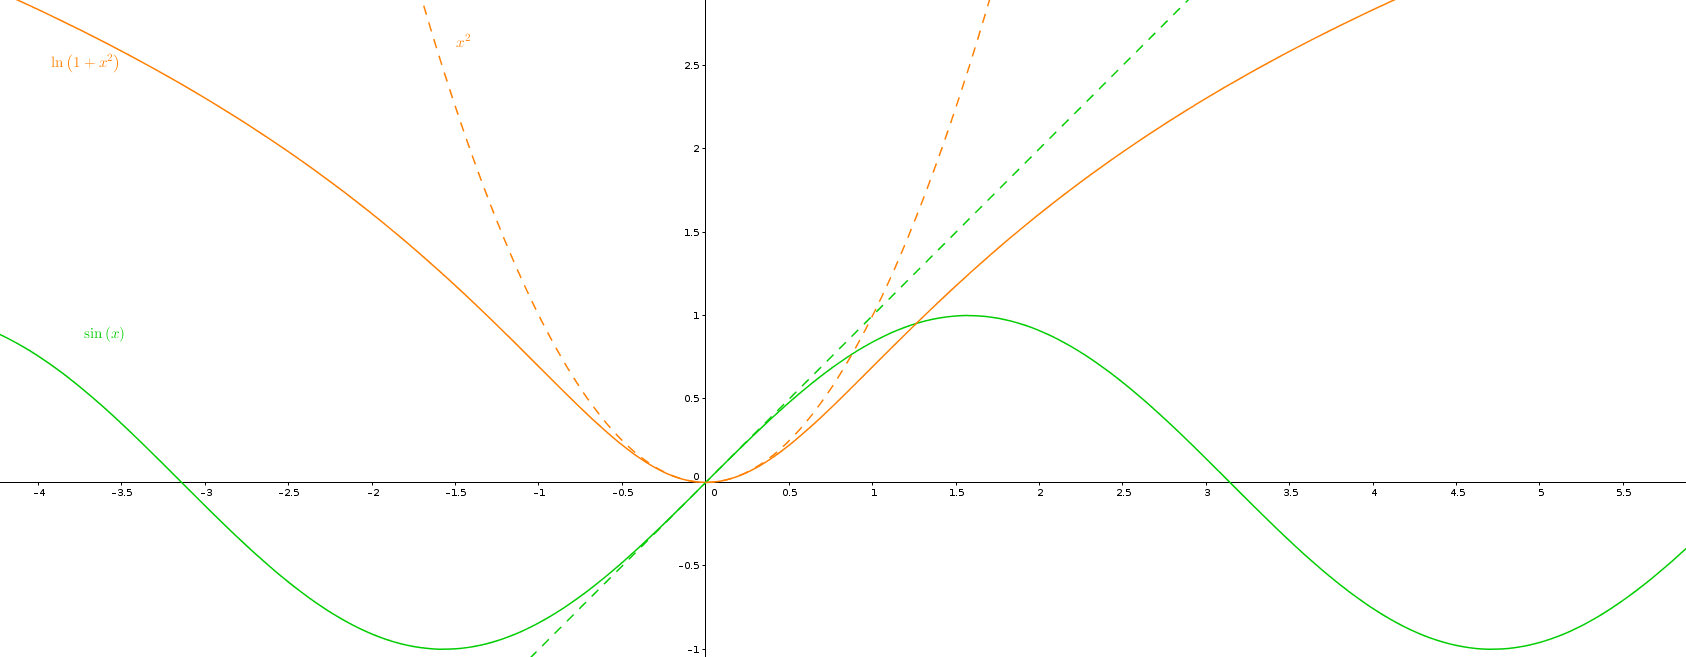
\includegraphics[width=500pt]{Images/SommeResteGrossier1}
	\end{figure}

	\begin{figure}[!h]
		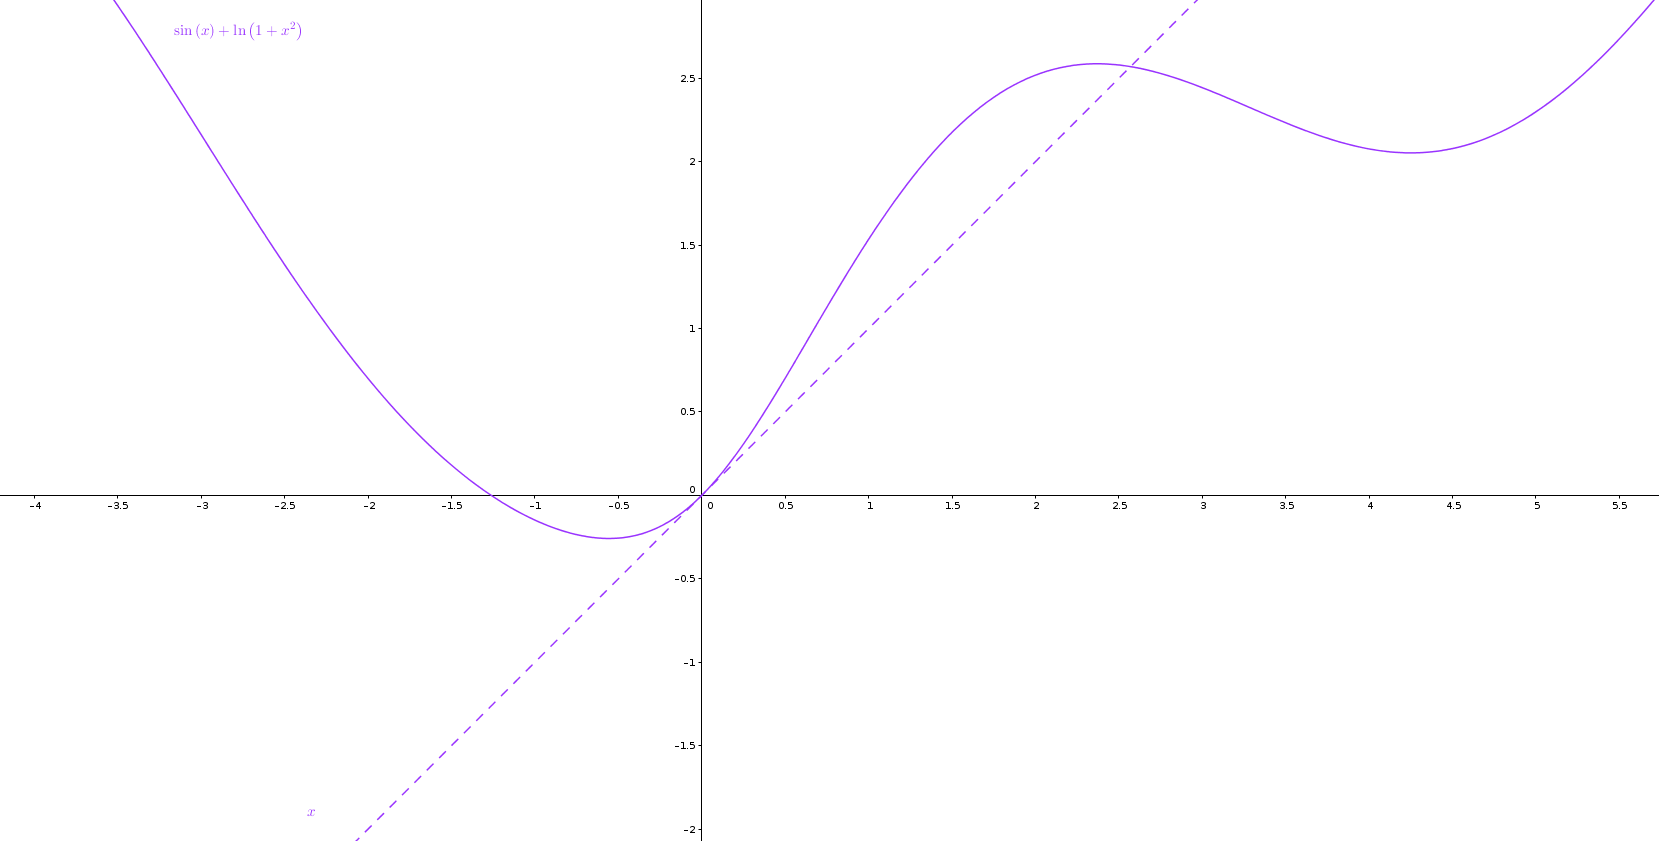
\includegraphics[width=500pt]{Images/SommeResteGrossier2}
		\caption{Somme de deux fonctions exprimées à l'aide de restes}
	\end{figure}
\end{enumerate}

\newpage

\paragraph{Remarque}
$f=o_a(1) \Longleftrightarrow \lim\limits_{a} \frac{f}{1} = 0 \Longleftrightarrow \lim\limits_{a} f = 0$.

\subsection{Équivalence}

\paragraph[Définition]{}
En $a$, $f$ et $g$ sont équivalentes en $a$ si et seulement si $f=g+o_a(g)$, noté $f \sim_a g$
Plus simplement, si $g$ ne s'annule pas au voisinage de $a$, $\displaystyle f \sim_a g \Leftrightarrow \lim_a \frac{f}{g}=1$.

\paragraph{Exemples}
\begin{enumerate}
	\item En $+ \infty$, $e^x + x^{2016} \sim e^x$ car $x^{2016}=o(e^x)$
	
	\item Si le développement limité de $f$ en $0$ à l'ordre $n$ est $f(x)=P(x)+o(x^n)$, alors $f(x) \sim P(x)$, par exemple $sin(x)=x-\frac{x^3}{6}+o(x^4)$, donc $sin(x) \sim x-\frac{x^3}{6}$.
	
	\item En $+\infty$, $ln(P(x)) \sim d \cdot ln(a_dx)$ avec $P = a_d X^d + a_{d-1}X^{d-1} + ... + a_0$ car $P(x) = a_d x^d + o(x^d)$ et $ln(P(x))=ln(a_d x^d(1+o(1)))=ln(a_dx^d)+ln(1+o(1)) \sim d \cdot ln(a_d x)$
\end{enumerate}

\paragraph{Propriétés}
\begin{enumerate}
	\item La relation d'équivalence est compatible avec la multiplication
	$$\left. \begin{array}{c c}
		f \sim_a g \\
		\phi \sim_a \psi \\
	\end{array} \right\} \Longrightarrow f \phi \sim_a g \psi$$
	
	\item La relation d'équivalence n'est généralement pas compatible avec la somme
	$$\left. \begin{array}{c c}
			x^2 + x\sim_{+\infty} x^2 \\
			-x^2 \sim_{+\infty} -x^2 \\
		\end{array} \right\} \nRightarrow x \sim_{+\infty} 0$$
	
	\paragraph{Attention}
	 Si $f \sim_a g$, alors on n'a pas nécessairement  $\lim\limits_{a} (f-g) = 0$, par exemple en $+\infty$, $x+1 \sim x$ mais $(x+1)-x=1$. Tout ce que l'on peut affirmer est que $f-g=o(f)=o(g)$.
	 
	 Cependant, cela est vrai si $\displaystyle \lim\limits_{a} f = l$ existe et est fini : $f$ et $g$ ont nécessairement la même limite, d'où $f-g=l+o_a(1)-(l+o_a(1))=o_a(1)$.
	
	\item La relation d'équivalence n'est généralement pas stable par dérivation : $1+2x \sim_0 1+x \nRightarrow 2 \sim_0 1$
	
	\item La relation d'équivalence n'est généralement pas compatible avec la composition à gauche : $x+1 \sim_{+\infty} x \nRightarrow e^x \sim_{+\infty} e^{x+1}=e\cdot e^x$.
	
	Certaines fonctions préservent cependant l'équivalence :
	\paragraph{Exercice}
	Soient $f$ et $g$ équivalentes en $a$, et soit $\alpha \ne 0$, montrez que $f^\alpha \sim_a g^\alpha$.
	
	En supposant à présent que $f \ne 0$ au voisinage de $a$, montrez $ln(f) \sim_a ln(g)$.
	
	\paragraph{Solution}
	$f^\alpha = (g+o(g))^\alpha = (g(1+o(1)))^\alpha=g^\alpha (1+o(1))^\alpha$, et comme $\lim\limits_{a} (1+o(1))^\alpha = 1$, on en déduit $f^\alpha \sim_a g^\alpha$
	
	$ln(f)=ln(g+o(g))=ln(g(1+o(1)))=ln(g)+ln(1+o(1))$, sachant $\lim\limits_{a} ln(1+o(1))=0$, on déduit $ln(f) \sim_a ln(g)$
	
	\item La relation d'équivalence est en revanche compatible avec la composition à droite sous certaines conditions :
		$$\left. \begin{array}{c c}
				f \sim_b g \\
				\lim\limits_{a} u=b\\
			\end{array} \right\} \Rightarrow f \circ u \sim_a g \circ u$$
	
	En pratique, cela signifie que l'on peut effectuer un changement de variable tant que la limite de celle-ci reste la même.
	
	Par exemple, en $0$ on a $ln(1+x) \sim x$, et en posant $u=\frac{1}{x}$, on obtient en $+\infty$ $ln(1+u)\sim u$, c'est à dire $ln\left(1+\frac{1}{x}\right) \sim \frac{1}{x}$.
	
	\paragraph{Remarque}
	L'équivalence est très adapté à la simplification d'un quotient ou produit, par exemple l'hideuse expression
	$$\frac{\left(n \, sin \left(\frac{1}{n}\right)\right)\left(\displaystyle \sum_{k=1}^{42} n^k + e^n\right)}{e^{n}} \left(\sqrt{n} + ln^7(n)\right)$$
	
	peut être remplacée selon le contexte (par exemple pour un calcul de limite) par un équivalent en $+\infty$ :
	
	$$\sqrt{n}$$
\end{enumerate}

\subsection{Domination}

\paragraph[Définition]{}
$g$ domine $f$ au voisinage de $a$, noté $f=O_a(g)$ (notation de Landau) ou $f \ll g$ (notation de Vinogradov), si et seulement s'il existe une constante $C \geqslant 0$ telle que pour $x$ assez proche de $a$, $|f(x)| \leqslant C|g(x)|$.

On utilise cette relation pour indiquer que \textit{$f$ ne croît pas plus vite que $g$}.

\paragraph{Exemples}
\begin{enumerate}
	\item $4x^5=O_{+\infty}(x^5)$
	
	\item Les grands $O$ sont utilisés pour exprimer la complexité d'un algorithme; on peut estimer le nombre d'étapes de calculs exécutées dans le pire des cas.
	
	Par exemple celle de l'algorithme du \textit{tri à bulle} (ou \textit{tri par propagation}), pour trier un tableau de $n$ éléments $(e_i)_{1 \leqslant i < n}$.
	
	A chaque étape $1 \leqslant k \leqslant n-1$, on parcourt le tableau en faisant varier $i$ de $k$ à $n-1$ afin d'échanger tout élément $e_i$ et $e_{i+1}$ si on a $e_i > e_{i+1}$.
	
	On effectue moins de $n^2$ échanges, c'est à dire $O(n^2)$ échanges, et le nombres d'instructions utilisées pour implémenter l'algorithme ne change pas ce grand $O$ car la relation de domination est stable par multiplication par une constante non-nulle (comme pour la prépondérance).
	
	\item $x \cdot sin(x) = O_{+\infty}(x)$
\end{enumerate}

\paragraph{Remarque}
Si $f=o(g)$, alors $f=O(g)$

\paragraph{Attention aux composition de fonctions}
Si on a $f < g$ et $h$ croissante, alors on a $h \circ f = O(h \circ g)$, mais l'implication $f=O(g) \Longrightarrow h \circ f = O(h \circ g)$ est fausse !

Par exemple en $+\infty$, $ln(x)=O\left(\frac{1}{2}ln(x)\right)$

et $exp$ est croissante, mais on n'a pas $x = O(\sqrt{x})$.

\section{Exercices}

\subsection{Comparaison de suites et fonctions}

\begin{enumerate}
\item Les assertions suivantes sont elles vraies ou fausses ?
\begin{enumerate}
	\item $n + 1 \sim_{+\infty} n$ donc $e^{n+1} \sim_{+\infty} e^n$.
	
	\item $x + x^2 \sim_0 x+3x^2$ donc $e^{x + x^2} \sim_0 e^{x + 3x^2}$
	
	\item $1+x \sim_0 1+x^2$ donc $ln(1+x^2) \sim_{0} ln(1+x)$
	
	\item $ln(x^2+sin (x)) \sim_{+\infty} 2x$
	
\end{enumerate}

\textit{Morale} : Soyez prudent avec les compositions d'équivalents.

A moins de chercher à simplifier un produit/quotient ou d'effectuer un changement de variable (sous-entendu dire que $sin\left(\frac{1}{n}\right) \sim_{+\infty} \frac{1}{n}$ sachant $sin(x) \sim_0 x$), je conseille de passer par les développements limités afin de contrôler le reste (le petit $o$).

\item Soient $f$ et $g$ définies au voisinage de $a \in \overline{\mathbb{R}}$, donnez une condition nécessaire et suffisante sur $f-g$ pour que $e^f \sim_a e^g$.

\item
Calculez $\displaystyle \lim_{x \to 0}cos(x)^{ln|x|}$

\item On peut facilement montrer $\sqrt{x^2+3x+5}\sim_{+\infty}x+\frac{3}{2}+\frac{11}{8x}$.

On cherche à savoir "à quelle vitesse" ces deux valeurs se rapprochent : trouvez un équivalent de $\sqrt{x^2+3x+5}-(x+\frac{3}{2}+\frac{11}{8x})$

\item Soit $m \in \mathbb{N}^*$, montrer $n(n-1)...(n-m+1) \sim n^m$

\item Donner des équivalent des expressions suivantes : 
\begin{enumerate}
	\item $\frac{2^n + 3^n}{n^2+ln(n)+5^n}$

	\item $arccos\left(\frac{n-1}{n}\right)$
	
	\textit{Indication :} utiliser $cos(h) \sim_0 1 - \frac{h^2}{2}$
\end{enumerate}

\item
Soit $c > 0$ une constante.
\begin{enumerate}
\item Montrer qu'en $+\infty$, $ln(x+c) \sim ln(x)$ et $\sqrt{x+c} \sim \sqrt{x}$.

\item Soit $f$ dérivable sur $\mathbb{R}$, à l'aide du théorème des accroissements finis, montrer que si $\lim\limits_{+\infty} f' = 0$, alors pour toute constante $c$ on a en $+\infty$, $f(x) \sim f(x+c)$.
\end{enumerate}

\item \textit{Exercice 4 de l'examen de MM3 du 7 janvier 2016 :}
\begin{enumerate}
	\item Montrer que la série de terme général $u_n=\frac{(-1)^n}{ln(1+\sqrt{n})}$ converge, mais ne converge pas absolument.
	
	\item Déterminer la nature de la série de terme général $u_n = \left\{ \begin{array}{c @{,} c}
 		1/n & $si $n$ est un carré$ \\
		1/n^2 & $sinon$\\
	\end{array} \right.$
	
	\item Soient $\displaystyle u_n = \frac{1}{n! 3^n} \prod_{k=1}^{n}(3k-2)$ et $v_n=\frac{1}{n^{3/4}}$, montrer que pour $n$ assez grand on a $\frac{u_{n+1}}{u_n} \geqslant \frac{v_{n+1}}{v_n}$. En déduire que $\sum u_n$ diverge.
	
	\textit{Indication} : faire un développement limité de $\frac{u_{n+1}}{u_n}$ et $\frac{v_{n+1}}{v_n}$.
\end{enumerate}

\item Étudier la convergence des séries numériques de termes généraux suivants
\begin{enumerate}
	\item $sin \left(\frac{n^2+n}{n} \pi\right)$
	
	\textit{Indication} : utiliser la formule d'addition pour le sinus $sin(a+b)=sin(a)cos(b)+sin(b)cos(a)$
	
	\item $\frac{1}{n^{1+\frac{1}{\sqrt{n}}}}$
\end{enumerate}

\item On cherche un équivalent de $ln(n!)$ quand $n$ tends vers $+\infty$.
\begin{enumerate}
	\item Montrez que $\displaystyle \int_0^1 ln$ est une intégrale impropre convergente et calculez sa valeur.
	
	\item Justifiez que $\displaystyle \lim\limits_{n} ~ \frac{1}{n}(ln(n!) - n \cdot ln(n)) = \int_{0}^{1} ln$
	
	\textit{Indication} : Développez $ln(n!)$ puis utilisez une somme de Riemann.
	
	\item Donnez un équivalent de $ln(n!)-n \cdot ln(n)$.
	
	Concluez que $ln(n!) \sim n \cdot ln(n)$.
\end{enumerate}

\end{enumerate}

\subsection{Séries de fonctions et séries entières}

\begin{enumerate}
\item \textit{Exercice 3 de l'examen de MM4 du 24 mai 2016 :}

On définit la suite $\textbf{f}=(f_n)_{n \in \mathbb{N}^*}$ avec pour tout $n > 0$, $f_n : [0, \frac{\pi}{2}] \longrightarrow \mathbb{R}, ~ x \longmapsto n sin(x) cos^n(x)$

\begin{enumerate}
	\item Pour chaque $x \in [0, \frac{\pi}{2}],$ calculer $\displaystyle \lim\limits_{n} f_n(x)$
	\item Calculer $\displaystyle I_n=\int_0^{\frac{\pi}{2}}f_n$ puis $\lim\limits_{n} I_n$
	\item La suite $(f_n)_{n \in \mathbb{N}^*}$ converge-t-elle uniformément sur $[0, \frac{\pi}{2}]$ ?
	\item Montrer que $(f_n)_{n \in \mathbb{N}^*}$ converge uniformément sur $[a,b]$ avec $0 < a < b \leqslant \frac{\pi}{2}$
\end{enumerate}

\paragraph{Rappel} Pour montrer que $\displaystyle \sum f_n$ converge uniformément on peut entre autre :
\begin{itemize}
	\item montrer qu'elle converge normalement, c'est à dire démontrer que $\displaystyle \sum ||f_n||_{\infty}$ converge.
	
	\item si la série converge simplement vers une fonction $f$ et si $f_n$ est de la forme $f_n=(-1)^n g_n$ avec $g_n$ positif (ou négatif) pour tout $n$ et que $||f_n||_{\infty}$ tend vers 0, utiliser le critère d'Abel pour montrer $\displaystyle \left|\left| f-\sum f_n\right|\right|_{\infty} \leqslant ||f_{n+1}||_{\infty}$.
\end{itemize}

Pour montrer au contraire qu'elle n'est \textit{pas} convergente, on peut tenter
\begin{itemize}
	\item de montrer que $\displaystyle ||f-\sum f_n||_{\infty}$ ne tend pas vers $0$.
	
	\item de raisonner par l'absurde en utilisant la préservation des dérivées / intégrales / continuité par la convergence uniforme.
\end{itemize}

\item \textit{Exercice 5 de l'examen de MM4 du 24 juin 2015}

On définit la suite $\textbf{f} = (f_n)_{n \in \mathbb{N}^*}$ avec $f_n : \mathbb{R} \longrightarrow \mathbb{R}$ et $f_n(x)=n x^2 e^{-x \sqrt{n}}$, ainsi que la série de fonctions $\displaystyle \sum_{n > 0}f_n$

\begin{enumerate}
	\item Étudier la convergence simple sur $\mathbb{R}$ de $\displaystyle \sum_{n > 0} f_n$ en distinguant les cas $x < 0$ et $x \geqslant 0$.
	
	\textit{Indication :} Rappelez vous que pour tout $\alpha, \beta, \gamma > 0$, $e^{-\alpha n^\beta}=O(n^{-\gamma})$.
	
	\item Soit $a > 0$, la série de fonctions converge-t-elle normalement sur $A= [a, +\infty]$ ?
	
	\item Converge-t-elle normalement sur $\mathbb{R}_+$ ?
	
	\item Converge-t-elle uniformément sur $\mathbb{R}_+$ ?
	
	\item Soit $h : A \longrightarrow \mathbb{R}$ définie par $\displaystyle h(x)=\sum_{n = 1}^{\infty}f_n(x)$, $h$ est elle continue ?
\end{enumerate}

\newpage
\item \textit{Exercice 5 de l'examen de MM4 du 24 mai 2016 :}

On définit la suite $\textbf{f}=(f_n)_{n \in \mathbb{N}^*}$ avec pour tout $\displaystyle n > 0$, $f_n : \mathbb{R} \longrightarrow \mathbb{R}$ et $f_n(x) = \frac{1}{n^2} arctan(nx)$.

\paragraph{Rappel}
la fonction $arctan$ est dérivable sur $\mathbb{R}$ de dérivée $arctan'(x)=\frac{1}{1+x^2}$, strictement croissante, impaire et telle que $\displaystyle \lim\limits_{+\infty} arctan = \frac{\pi}{2}$.

\begin{figure}[!h]
	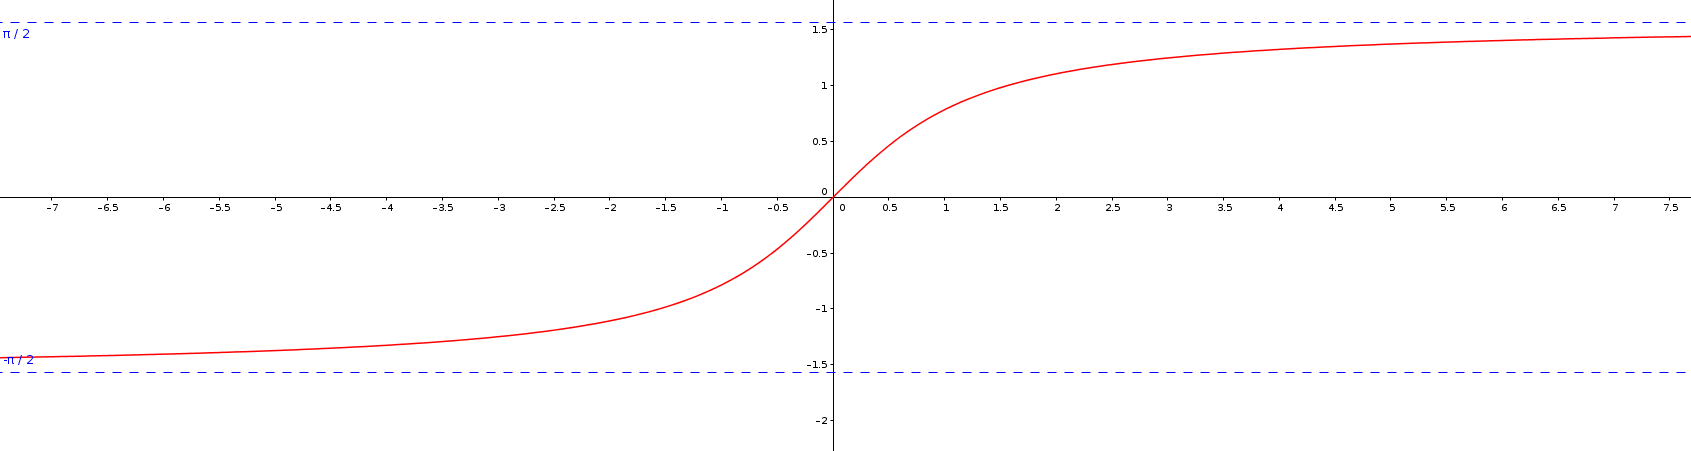
\includegraphics[width=350pt]{Images/Arctan}
	\caption{La fonction arctan}
\end{figure}

\begin{enumerate}
	\item Montrer que $\displaystyle f : \mathbb{R} \longrightarrow \mathbb{R}, ~ x \longmapsto \sum_{n=0}^{\infty}f_n(x)$ est continue sur $\mathbb{R}$.
	
	\item Montrer que pour tout $a > 0$, $f$ est dérivable sur $]-\infty, -a] \cup [a, +\infty[$.
	
	\item En conclure que $f$ est dérivable sur $\mathbb{R}^*$.
\end{enumerate}

\item Calculer les rayons de convergence $R$ des séries entières suivantes:
\begin{enumerate}
	\item $\displaystyle \sum_{n > 0}\frac{ln(n)}{ln(n+1)}z^n$
	\item $\displaystyle \sum_{n > 0}\frac{ln(n)}{n^2}z^{2n}$
	\item $\displaystyle \sum_{n \geqslant 0}a_n z^{2n}$ avec $R'$ le rayon de convergence de $\displaystyle \sum_{n \geqslant 0}a_n z^n$
	\item $\displaystyle \sum_{n > 0}sin \left(\frac{1}{\sqrt{n}}\right) z^n$ et étudier la convergence en $\pm R$
	\end{enumerate}

\paragraph{Rappel} La série entière $\sum a_n z^n$ n'est qu'un cas particulier de série ! On peut encore utiliser les critères de séries numériques, notamment les équivalents / petits o / grand O, critères de d'Alembert / Cauchy / Abel.

Par exemple, si $a_n \sim b_n$, pour un $z$ fixé $\sum a_n z^n$ converge \textit{si et seulement si} $\sum b_n z^n$ converge, ainsi les deux séries ont le même rayon de convergence.

Ou encore, si $a_n z^n = O\left( \frac{1}{n^\alpha}\right)$ avec $\alpha > 1$, alors $\sum a_n z^n$ converge pour tout $z$, ce qui signifie que son rayon de convergence est $R= +\infty$.

\item Démontrer que si $l = \lim\limits_{n} \left|\frac{a_n}{a_{n+1}}\right|$ existe, alors le rayon de convergence de $\sum a_nz^n$ vaut $l$.

\paragraph{Rappel} La série entière $\sum P(n)a_n z^n$ où $P$ est un polynôme a le même rayon de convergence que $\sum a_n z^n$. C'est pourquoi pour toute fraction rationnelle $F$, $\sum F(n) a_n z^n$ a le même rayon de convergence que $\sum a_n z^n$.

En effet si $F = \frac{P(n)}{Q(n)}$, alors $\sum F(n) a_n z^n = \sum \frac{P}{Q} a_n z^n$ a le même rayon de convergence que $\sum Q(n)\frac{P(n)}{Q(n)} a_n z^n = \sum P(n) a_n z^n$ qui a le même rayon de convergence que $\sum a_n z^n$.

\item Soit $f : \mathbb{R} \longrightarrow \mathbb{R}$ dérivable en tout ordre en $0$ et telle qu'il existe $M \geqslant 0$ vérifiant $\forall n \in \mathbb{N}, ~ ||f^{(n)}||_{\infty} \leqslant M$, montrer que le développement en série entière autour de $0$ de $f$ a un rayon de convergence infini.

En déduire le rayon de convergence du développement en série entière de $cos$ et $sin$.

\end{enumerate}

\section{Correction}

\subsection{Comparaison de suites et fonctions}

\begin{enumerate}
\item
\begin{enumerate}
	\item $\frac{e^{n+1}}{e^n}=e \ne 1$. Faux.
	\item Les deux expressions tendent vers une même limite non-nulle. Vrai.
	\item $ln(1+x) = x + o(x)$ et $ln(1+x^2)=x^2+o(x^2)$, mais $\displaystyle \lim\limits_{x \to 0} \frac{x+o(x)}{x^2+o(x^2)}= \infty$. Faux.
	\item $ln(x^2+sin(x))=ln\left(x^2\left(1+\frac{sin(x)}{x^2}\right)\right)=ln(x^2)+ln\left(1+\frac{sin(x)}{x^2}\right)$
	
	$ln(x^2+sin(x))=2ln(x)+\frac{sin(x)}{x^2}+o\left(\frac{1}{x^2}\right) \sim 2ln(x)$. Vrai.
\end{enumerate}

\item $e^f \sim_a e^g \Leftrightarrow \lim\limits_{a} \frac{e^f}{e^g} = 1 \Leftrightarrow \lim\limits_{a} e^{f-g} = 1 \Leftrightarrow \lim\limits_{a}(f-g)=0$.

\item La fonction $x \longmapsto cos(x)^{ln |x|}$ est paire, on se contentera donc d'étudier la limite en $0$ à droite.

$cos(x)^{ln (x)}=exp(ln(cos(x)) ln(x))$

Or $cos(x) = 1 - \frac{x^2}{2}+ o(x^2)$

Donc, $cos(x)^{ln(x)} = exp(ln((1 - \frac{x^2}{2} + o(x^2)) \cdot ln(x))$

$cos(x)^{ln(x)} = exp((-\frac{x^2}{2}+o(x^2)) \cdot ln(x))=exp(-\frac{x}{2} \cdot x \, ln(x) + o(x^2ln(x))$

Enfin, d'après le théorème des croissances comparées, $x \, ln(x) \to 0$, donc $cos(x)^{ln(x)} \to 1$

\item $\sqrt{x^2+3x+5}=|x|\sqrt{1+\frac{3}{x}+\frac{5}{x^2}}$

On connaît le développement limité $\sqrt{1+h}=1+\frac{h}{2}-\frac{h^2}{8}+\frac{h^3}{16} + o(h^3)$

d'où $\sqrt{1+\frac{3}{x}+\frac{5}{x^2}} = 1+\frac{1}{2}(\frac{3}{x}+\frac{5}{x^2})-\frac{1}{8}(\frac{3}{x}+\frac{5}{x^2})^2+\frac{1}{16}(\frac{3}{x}+\frac{5}{x^2})^3 + o(\frac{1}{x^3})$

$\sqrt{1+\frac{3}{x}+\frac{5}{x^2}} = 1+(\frac{3}{2x}+\frac{5}{2x^2})-\frac{1}{8}(\frac{9}{x^2}+\frac{30}{x^3}+o(\frac{1}{x^3}))+\frac{1}{16}(\frac{27}{x^3}+o(\frac{1}{x^3})) + o(\frac{1}{x^3})$

$\sqrt{1+\frac{3}{x}+\frac{5}{x^2}}=1+\frac{3}{2x}+\frac{11}{8x^2}+\frac{33}{16x^3}+o(\frac{1}{x^3})$

Ainsi, $\sqrt{x^3+3x+5} \sim x + \frac{3}{2} + \frac{11}{8x} + \frac{33}{16x^2}$

Et $\sqrt{x^3+3x+5} - (x+\frac{3}{2} + \frac{11}{8x}) \sim \frac{33}{16x^2} $

\paragraph{Astuce} lorsqu'on calcule un développement limité à l'ordre $n$, on est amené à calculer des puissances de polynômes, ce qui est de plus en plus fastidieux au fur et à mesure que la puissance grandit.

Lors du calcul de $P(u)^m$, où $u$ est notre variable qui tend vers $0$, on se contente de calculer les termes de la forme $\alpha \cdot u^k$ avec $k < n$, le reste de l'expression sera (une somme de) $o(u^n)$.

On peut réutiliser cette expression malicieusement calculée pour trouver $P(u)^{m+1}$.

\item Si on développe $n(n-1)...(n-m+1)$, on obtient $n^m + a_{m-1} n^{m-1} + ... + a_1 n$, et on sait que pour tout $1 \leqslant k \leqslant m-1$, $n^k=o(n^m)$.

Alors $n(n-1)...(n-m-1)=n^m+m \cdot o(n^m) = n^m + o(n^m) \sim n^m$

\paragraph{Attention}
Cela marche \textit{uniquement} car $m$ est une constante : $o(n^m)$ est stable par multiplication par une constante.

\item
\begin{enumerate}
\item $2^n = o(3^n)$, donc $2^n+3^n \sim 3^n$

$n^2, ln(n)=o(5^n)$, donc $n^2+ln(n) + 5^n \sim 5^n$

Ainsi $\frac{2^n+3^n}{n^2+ln(n)+5^n} \sim \left(\frac{3}{5}\right)^n$

\item $\frac{n-1}{n} \to 1$ donc $u_n \to 0$, on peut alors affirmer $cos(u_n) \sim 1 - \frac{u^2_n}{2}$

Or $cos(u_n)=\frac{n-1}{n}$, d'où $1-\frac{1}{n} \sim 1- \frac{u^2_n}{2}$ et donc $u_n \sim \sqrt{\frac{2}{n}}$

\end{enumerate}

\item
\begin{enumerate}
	\item $ln(x+c)=ln\left(x\left(\frac{c}{x}+1\right)\right)=ln(x)+ln\left(1+\frac{c}{x}\right) \sim ln(x)$
	
	Ou bien $\lim\limits_{x \to +\infty} \frac{ln(x+c)}{ln(x)}=\lim\limits_{x \to +\infty} \frac{x}{x+c}=1$ d'après la règle de l'Hôpital.
	
	$\sqrt{x+c}=\sqrt{x\left(\frac{c}{x}+1\right)}=\sqrt{x} \cdot \sqrt{1+\frac{c}{x}} \sim \sqrt{x}$
	
	Ou bien $\lim\limits_{x \to +\infty} \frac{\sqrt{x+c}}{\sqrt{x}}=\lim\limits_{x \to +\infty} \sqrt{\frac{x+c}{x}}=\lim\limits_{x \to +\infty} \sqrt{1+\frac{c}{x}}$
	
	\item D'après le théorème des accroissements finis, pour tout $x > 0$ il existe un $\alpha_x \in ]x, x+c[$ tel que $\frac{f(x+c)-f(x)}{(x+c)-x}=\frac{f(x+c)-f(x)}{c}=f'(\alpha_x)$
	
	C'est pourquoi, si $\lim\limits_{+\infty}f'=0$, alors $\lim\limits_{x \to +\infty} f(x+c)-f(x)=0$
	
	Ainsi $f(x+c) \sim f(x)$
	
	\begin{figure}[!h]
		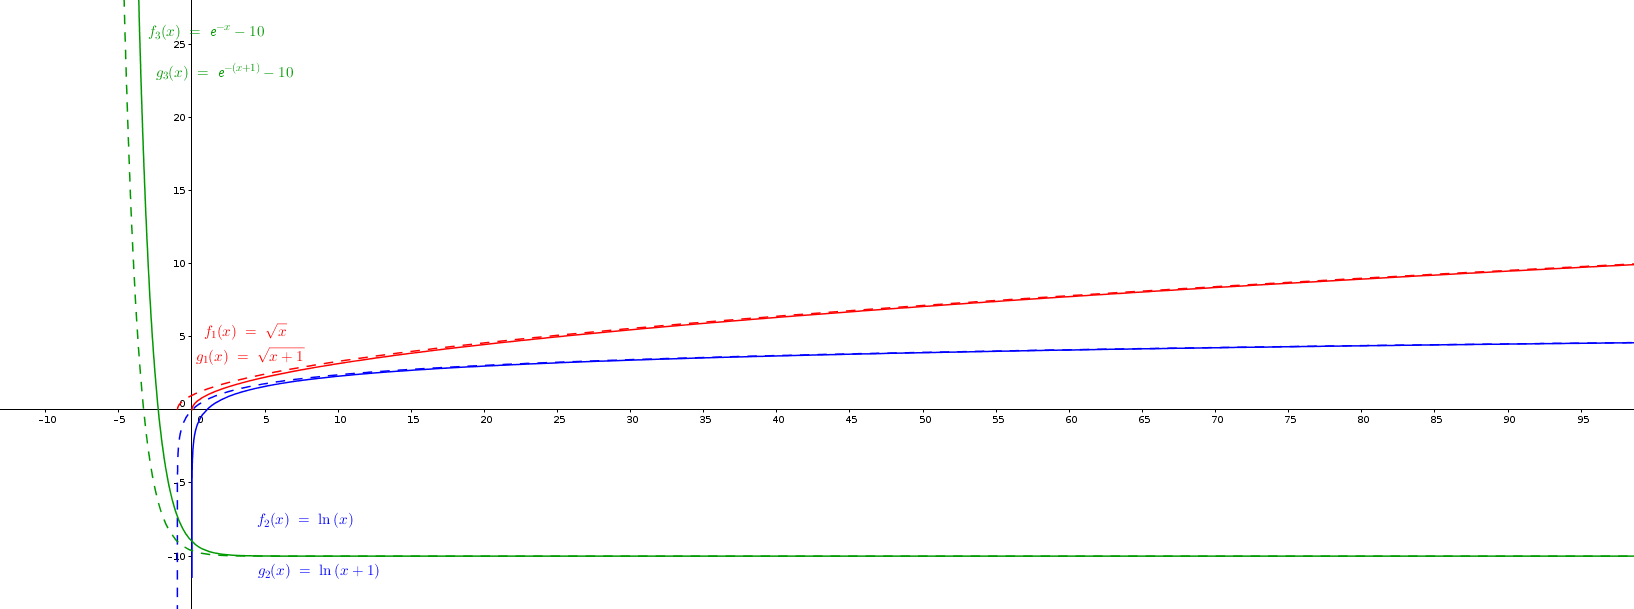
\includegraphics[width=350pt]{Images/DeriveNulle}
		\caption{Exemple de trois fonctions dont la dérivée tend vers 0}
	\end{figure}
\end{enumerate}

\item
\begin{enumerate}
	\item $\frac{1}{ln(1+\sqrt{n})}$ est positive, décroissante et tend vers $0$, donc d'après le critère d'Abel la série $\sum u_n$ converge.
	
	Cependant $ln(1+\sqrt{n}) \sim ln(\sqrt{n})=\frac{1}{2}ln(n)$, de plus pour $n$ assez grand, $ln(n) < n$ d'où $\frac{2}{ln(n)} > \frac{2}{n}$ et alors $\sum u_n$ ne converge pas absolument.
	
	\item Pour tout $n$, $u_n$ est de la forme $\frac{1}{k^2}$ avec $k \in \mathbb{N}^*$, tout $\frac{1}{k^2}$ apparaît au plus deux fois, on a alors la majoration $\displaystyle \sum_{n=1}^{N} u_n \leqslant 2\sum_{n = 1}^{N} \frac{1}{n^2}$ et donc $\sum u_n$ converge.
	
	\item On cherche à montrer que $\sum u_n$ diverge, sachant $u_n$ non-nulle pour tout $n$, il suffirait de montrer qu'à partir d'un certain rang elle est largement croissante, c'est à dire que pour $n$ assez grand $\frac{u_{n+1}}{u_n} \geqslant 1$.
	
	On sait que $(n+1)^{3/4} \sim n^{3/4}$ et que $(v_n)$ est croissante, donc $\frac{v_{n+1}}{v_n} \geqslant 1$.
	
	Ainsi, si on montre que pour $n$ assez grand $\frac{u_{n+1}}{u_n} \geqslant \frac{v_{n+1}}{v_n}$ on aura $\frac{u_{n+1}}{u_n} \geqslant 1$.
	
	$$\frac{u_{n+1}}{u_n} \geqslant \frac{v_{n+1}}{v_n} \Longleftrightarrow \frac{3n+2}{3(n+1)} \geqslant \left(\frac{n}{n+1}\right)^{3/4}$$
	
	$$\frac{u_{n+1}}{u_n} \geqslant \frac{v_{n+1}}{v_n} \Longleftrightarrow \left(1-\frac{1}{3n+2}\right) \geqslant \left(1-\frac{1}{n+1}\right)^{3/4}$$
	
	$$\frac{u_{n+1}}{u_n} \geqslant \frac{v_{n+1}}{v_n} \Longleftrightarrow 1 - \frac{1}{3n} + o\left(\frac{1}{n}\right) \geqslant 1 - \frac{3}{4n} + o\left(\frac{1}{n}\right)$$
	
	$$\frac{u_{n+1}}{u_n} \geqslant \frac{v_{n+1}}{v_n} \Longleftrightarrow \frac{1}{3n} \leqslant \frac{3}{4n} +o\left(\frac{1}{n}\right)$$
	
	$\frac{1}{3} < \frac{3}{4}$ donc pour $n$ assez grand on a bien $\frac{u_{n+1}}{u_n} \geqslant \frac{v_{n+1}}{v_n}$ !
\end{enumerate}

\item
\begin{enumerate}
	\item $sin\left(\frac{n^2+1}{n}\pi\right)=sin\left(n\pi+\frac{\pi}{n}\right)=sin(n\pi)cos\left(\frac{\pi}{n}\right) + cos(n\pi)sin\left(\frac{\pi}{n}\right)$
	
	$sin\left(\frac{n^2+1}{n}\pi\right) = 0 \cdot cos\left(\frac{\pi}{n}\right) + (-1)^n sin\left(\frac{\pi}{n}\right)$
	
	$sin\left(\frac{n^2+1}{n}\pi\right) = (-1)^n sin\left(\frac{\pi}{n}\right)$
	
	$sin\left(\frac{n^2+1}{n}\pi\right) \sim (-1)^n \frac{\pi}{n}$
	
	$\sum \frac{(-1)^n}{n}$ converge, donc $\sum sin\left(\frac{n^2+1}{n}\pi\right)$ converge.
	
	\item
	$\frac{1}{n^{1+1/\sqrt{n}}} = \frac{1}{
	n} \cdot \frac{1}{n^\frac{1}{\sqrt{n}}} = \frac{1}{
		n} \cdot \frac{1}{e^{\frac{ln(n)}{\sqrt{n}}}} \sim \frac{1}{n}$ donc la série diverge.
\end{enumerate}

\item
\begin{enumerate}
	\item Soit $\epsilon > 0$, $\displaystyle \int_{\epsilon}^{1}ln = [x\cdot ln(x)-x]_\epsilon^1=-1-\epsilon\cdot ln(\epsilon)+\epsilon$
	
	$\displaystyle \int_0^1 ln = \lim\limits_{\epsilon \to 0} \int_{\epsilon}^{1} ln = -1$
	
	\item $ln(n!) - n \cdot ln(n) = \displaystyle \sum_{k=1}^{n} ln(k) - n \cdot ln(n)$
	
	$ln(n!) - n \cdot ln(n) = \displaystyle \sum_{k=1}^{n} (ln(k) - ln(n))$
	
	$ln(n!) - n \cdot ln(n) = \displaystyle \sum_{k=1}^{n} ln \left(\frac{k}{n}\right)$
	
	$\frac{1}{n} (ln(n!) - n \cdot ln(n)) = \frac{1}{n}\displaystyle \sum_{k=1}^{n} ln \left(\frac{k}{n}\right)$
	
	On se retrouve avec une somme de Riemann, on peut alors conclure que $\displaystyle \lim\limits_{n} \frac{1}{n} (ln(n!) - n \cdot ln(n)) = \int_0^1 ln = -1$
	
	\item $\displaystyle \lim\limits_{n} \frac{1}{n} (ln(n!) - n \cdot ln(n)) = \int_0^1 ln = -1$, c'est à dire :
	$$\frac{1}{n} (ln(n!) - n \cdot ln(n)) = -1 + o(1)$$
	
	$$ln(n!) - n \cdot ln(n) = -n + o(n)$$
	
	$$ln(n!) = n \cdot ln(n) - n + o(n)$$
	
	Ainsi, $ln(n!) \sim n(ln(n)-1)$, et plus grossièrement, $ln(n!) = n \cdot ln(n) + o(n \cdot ln(n)) \sim n \cdot ln(n)$
\end{enumerate}

\end{enumerate}

\subsection{Séries de fonctions et séries entières}

\begin{enumerate}

\item
\begin{enumerate}
	\item Si $x = 0, \frac{\pi}{2}$, alors $sin(x)cos(x) = 0$.
	
	Si $0 < x < \frac{\pi}{2}$, alors $0 < cos(x) = \alpha < 1$ et $f_n(x)=sin(x) \cdot n \alpha^n$, or $sin(x)$ est constant lorsque $n$ tend vers $\infty$ et $n \alpha^n \to 0$.
	
	C'est à dire $f_n \to 0$
	
	\item On connaît la dérivée de $cos^{n+1}(x)$ : c'est $-(n+1)sin(x)cos^n(x)$, et donc $$I_n = \int_{0}^{\frac{\pi}{2}}f_n = \int_{0}^{\frac{\pi}{2}}n sin(x) cos^n(x)$$
	
	$$I_n = - \int_{0}^{\frac{\pi}{2}}-\frac{n+1}{n+1} n sin(x) cos(x)^n$$
	
	$$I_n = -\frac{n}{n+1}\int_{0}^{\frac{\pi}{2}} - (n+1) sin(x) cos^n(x)$$
	
	$$I_n = - \frac{n}{n+1}[cos^{n+1}(x)]^{\frac{\pi}{2}}_0 = $$
	
	$$I_n=\frac{n}{n+1}$$
	
	On en déduit $\lim\limits_{n \to \infty} I_n = 1$
	
	\item La suite $\textbf{f}$ ne peut pas converger uniformément ; si c'était le cas on aurait $\displaystyle \lim\limits_{n} \int_{0}^{\frac{\pi}{2}}f_n = \int_{0}^{\frac{\pi}{2}} \lim\limits_{n}f_n$.
	
	Or d'une part $\displaystyle \lim\limits_{n} f_n = 0$ d'après (a) et $\displaystyle \int_{0}^{\frac{\pi}{2}} 0 = 0$, et $\displaystyle \int_{0}^{\frac{\pi}{2}} f_n = I_n \to 1$ d'après (b). Il y a contradiction.
	
	\item Pour $0 < a < x < b \leqslant \frac{\pi}{2}$, $|sin(x)| \leqslant 1$ et $|cos(x)| \leqslant |cos(a)| = \alpha < 1$
	
	Ainsi $|f_n(x)| < n \alpha^n$ pour tout $x \in [a, b]$ et donc $||f_n||_{\infty, [a,b]} \leqslant n \alpha^n$ qui tend vers 0 quand $n$ tend vers $\infty$.
\end{enumerate}

\item 
\begin{enumerate}
	\item
	\begin{itemize}
		\item Soit $x < 0$, $f_n(x) \to +\infty$, la série diverge sur $\mathbb{R}^*_-$.
		\item Soit $x \geqslant 0$, $e^{-x \sqrt{n}} = O(n^{-3})$ donc $f_n(x)=O(x^2 n^{-2})$, la série converge sur $\mathbb{R}_+$.
	\end{itemize}
	\item Calculons $||f_n||_{\infty, \mathbb{R_+}}$ pour tout $n > 0$ :
	
	$f_n$ est dérivable sur $A$, de dérivée $f'_n(x)=n (2x e^{-x\sqrt{n}}-\sqrt{n} \, e^{-x\sqrt{n}}x^2)=nxe^{-x\sqrt{n}}(2-x\sqrt{n})$
	
	$||f_n||_{\infty, A}=\left|f_n\left(\frac{2}{\sqrt{n}}\right)\right|=\frac{4}{e^2}$
	
	$\displaystyle \sum_{n > 0} f_n$ ne converge pas normalement sur $\mathbb{R}_+$.
	
	\paragraph{Astuce} Si on est face à une fonction $f$ de signe constant, dérivable et telle que $\lim\limits_{+\infty}f=0$ et dont la dérivée change de signe en un seul point $a$, on peut immédiatement dire que $\max~|f|=|f(a)|$, il est inutile de passer par un tableau de signe !
	
	\begin{figure}[!h]
		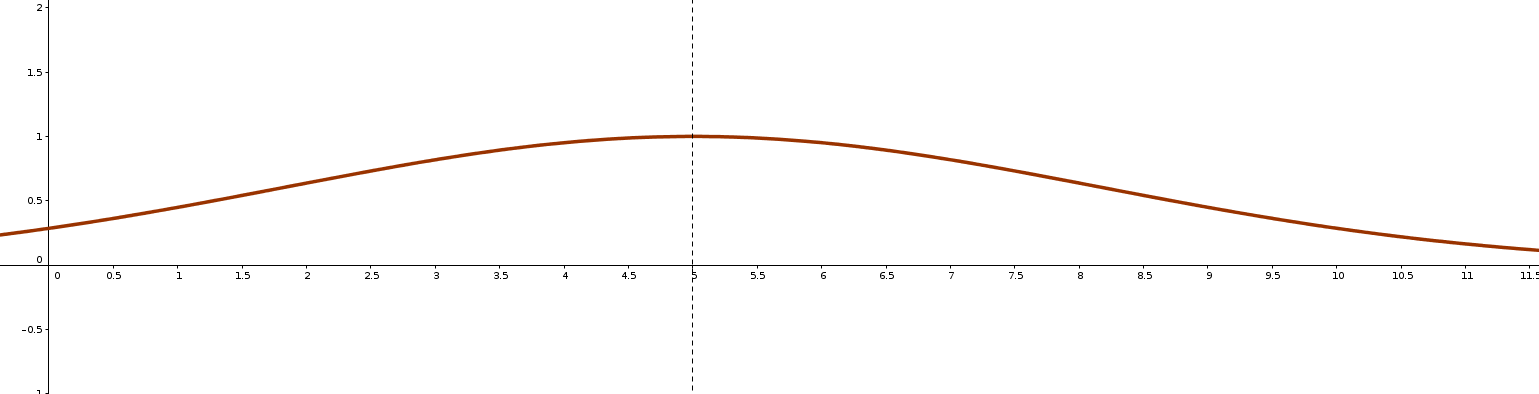
\includegraphics[width=350pt]{Images/max_liminfinini}
	\end{figure}
	
	\item Pour $n$ assez grand, $\frac{2}{\sqrt{n}} < a$, alors $||f_n||_{\infty, A}=\max |f_n|=f_n(a)$ car $f_n$ est décroissante sur $A$.
	
	Or comme on l'a vu en (a), $f_n(a)=O(n^{-2})$, donc $\displaystyle \sum f_n$ converge uniformément sur $A$.
	
	\item Chaque $f_n$ et donc $\displaystyle \sum_{k=1}^{n} f_n$ est continue sur $A$, d'où $h$ est continue sur $A$.
\end{enumerate}

\item
On notera $\displaystyle F_n = \sum_{k = 1}^{n}f_k$ la suite des sommes partielles.

\begin{enumerate}
	\item Pour tout $n > 0$, et pour tout $x \in \mathbb{R}$, $|f_n(x)| < \frac{\pi}{2n^2}$, d'où $||f_n||_{\infty} \leqslant \frac{\pi}{2n^2}$, et pour cette raison $\displaystyle \sum_{n > 0} f_n$ converge normalement, et donc uniformément.
	
	\item Chaque $f_n$ et donc $F_n$ et $f$ sont impaires, on se limitera donc à les étudier sur $A = [a, +\infty[$.
	
	Pour tout $n > 0$ et $x > a > 0$, $f'_n(x) = \frac{n}{n^2(1+n^2x^2)} = \frac{1}{n(1+n^2x^2)}$, donc $\displaystyle ||f'_n||_{\infty, A}=\sup_{x > a} |f'_n(x)| = \frac{1}{n(1+a^2n^2)} \sim_n \frac{1}{a^2 n^3}$.
	
	Pour la même raison que précédemment, $\displaystyle \sum_{n > 0}f'_n$ converge uniformément.
	
	On a à présent réuni les trois conditions suivantes :
	\begin{itemize}
		\item $F'_n$ converge uniformément sur $A$.
		\item Pour tout $n > 0$, $F_n$ est dérivable. 
		\item Il existe $x_0$ tel que $\displaystyle F_n(x_0)$ converge (car d'après (a) la série converge, mais on peut prendre par exemple $x_0 = 0$).
	\end{itemize}
	Ce qui implique que $\displaystyle \lim\limits_{n} F_n = f$ est dérivable sur $A$.
	
	Ainsi $f$ est dérivable sur $]-\infty, -a] \cup [a, +\infty[$.
	
	\item Pour tout $x > 0$, $f'(x)$ existe car d'après (b) $f$ est dérivable sur $]-\infty, -x] \cup [x, +\infty[$. De même pour $x < 0$.
	
	Ainsi, $f$ est dérivable sur $\mathbb{R}^*$.
\end{enumerate}

\paragraph{Remarque} On a travaillé sur $\mathbb{R}^*$ et pas sur $\mathbb{R}$ car pour $a=0$, $||f'_n||_{\infty, A}=\frac{1}{n(1+n^2a^2)}=\frac{1}{n}$ et on n'a plus que $\displaystyle \sum_{n > 0} f'_n$ converge normalement sur $A$.


\item
\begin{enumerate}
	\item Il est inutile d'appliquer le critère de d'Alembert : $ln(n+1) \sim ln(n)$ donc $a_n z^n \sim z^n$ et ainsi $\sum a_n z^n$ a le même rayon de convergence que $\sum z^n$ : $R=1$.
	
		
	\item Pour la série $S(z)=\displaystyle \sum_{n>0} \frac{ln(n)}{n^2}z^{2n}$, nous ne pouvons malheureusement pas appliquer la règle de d'Alembert car si on réécrit la série sous la forme $\sum a_n z^n$, tous les coefficients des puissances impaires seront nuls.
	
	On pose alors une nouvelle série entière $T(u)=\displaystyle \sum_{n > 0} \frac{ln(n)}{n^2} u^n$ avec $u=z^2$, dont on peut calculer le rayon de convergence : $R = \lim\limits_{n} \frac{ln(n)}{n^2} \cdot \frac{(n+1)^2}{ln(n+1)} = 1$
	
	$T(u)=S(z^2)$ converge pour $|z^2| < 1$ et diverge pour $|z^2| > 1$, ainsi le rayon de convergence de $S(z)$ est $1$.
	
	\item
	$sin\left(\frac{1}{\sqrt{n}}\right) \sim \frac{1}{\sqrt{n}}$
	
	En appliquant la règle de d'Alembert on trouve que le rayon de convergence est $1$.
	
	Étudions à présent la convergence en $\pm 1$ :
	
	$\sum sin\left(\frac{1}{\sqrt{n}}\right)1^n=\sum sin\left(\frac{1}{\sqrt{n}}\right)$ diverge car $sin\left(\frac{1}{\sqrt{n}}\right) \sim \frac{1}{\sqrt{n}}$
	
	En revanche, $\sum sin\left(\frac{1}{\sqrt{n}}\right)(-1)^n$ converge d'après le critère d'Abel sur les séries alternées car $sin\left(\frac{1}{\sqrt{n}}\right)(-1)^n \sim \frac{(-1)^n}{\sqrt{n}}$.
\end{enumerate}

\item Supposons que $\lim\limits_{n} \left|\frac{a_n}{a_{n+1}}\right|=l$ existe.

On considère la série entière $\sum a_n z^n$ comme une série numérique avec un paramètre $z$.

On applique le critère de d'Alembert pour savoir si $\sum a_n z^n$ converge : 

$$\lim\limits_{n} \left|\frac{a_n z^n}{a_{n+1} z^{n+1}}\right| = \lim\limits_{n} \left|\frac{a_n}{a_{n+1}}\right|\left| \cdot \frac{1}{z}\right| = \frac{l}{|z|}$$

D'après le critère de d'Alembert, $\sum a_n z^n$ converge si $\frac{l}{|z|} < 1$ (c'est à dire $l < |z|$) et diverge si $\frac{l}{|z|} > 1$ (c'est à dire $l > |z|$).

On en déduit $R = |l|$

\item Le développement en série entière de $f$ est $\displaystyle \sum \frac{f^{(n)}(0)}{n!}z^n$.

On veut montrer que le rayon de convergence est infini, c'est à dire que pour tout $z$ cette série converge, autrement dit que $\left|f(z) - \sum_{k=0}^{n} \frac{f^{(k)}(0)}{k!}z^k \right|$ tends vers $0$ quand $n$ tend vers l'infini.

Par chance, on sait majorer ce reste ! Grâce à l'inégalité de Taylor qui nous dit que celui-ci est inférieur ou égal à $\left|\frac{sup f^{(n)}}{n!}z^n\right|$.

On a supposé que pour tout $n$, $|sup f^{(n)}| \leqslant M$, ainsi on a que le reste est majoré par $M\frac{z^n}{n!}$ qui tend vers $0$ :

$$\frac{(n+1)!}{z^{n+1}} \cdot \frac{z^n}{n!} = \frac{z}{n+1} \to 0$$

On  peut donc majorer $M \frac{z^n}{n!}$ par une suite géométrique de raison strictement inférieure à $1$ en valeur absolue et donc tendant vers 1.

Le reste tend alors vers 0, la série a un rayon de convergence infini.

\end{enumerate}

\newpage

\tableofcontents

\end{document}